\section{Superficies dadas en forma paramétrica}

\begin{figure}[H] 
    \centering    
    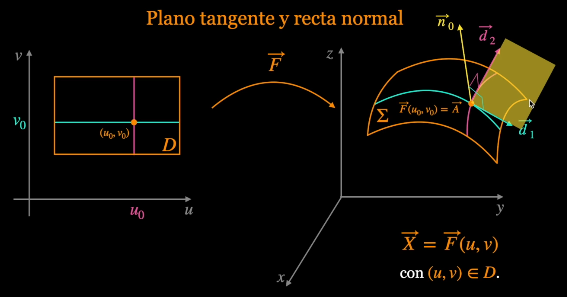
\includegraphics[width=0.6\textwidth]{img/ej-sup.png}
    \label{fig:ej-sup}
\end{figure}

Sea la superficie $\Sigma$ de ecuación $\vec{X} = \vec{F}(u,v)$ con $(u,v) \in D$.
Un punto $\vec{A} = \vec{F}(u_0, v_0)$ un punto regular de la superficie cuando $\vec{F}$ diferenciable en $(u_0, v_0)$ y $\vec{n_0} = \vec{F}'_u(u_0, v_0) \times \vec{F}'_v(u_0, v_0) \neq \vec{0}$.

\begin{itemize}
    \item Una ecuación para la recta normal a $\Sigma$ en el punto $\vec{A}$ es:
    $\vec{r}(t) = \vec{A} + t \, \vec{n_0}$, $t \in \mathbb{R}$.
    \item Una ecuación para el plano tangente a $\Sigma$ en el punto $\vec{A}$ es:
    $\vec{n_0} \cdot (\vec{X} - \vec{A}) = 0$.
\end{itemize}